\section{Program til skalaer}
\label{TestAfSkalaProgramSkala}
%
Programmet, som blev brugt til at præsentere skalaerne for testpersonerne, blev udviklet i \textit{Processing 3.3.6}, \parencite{WEB:Processing3}. Det bygger på et widget-bibliotek udviklet af Søren Krarup Olesen m.fl. som hedder \textit{PDPGUITest}. I programmet er der lavet klasser til blandt andet check bokse, radio knapper, sliders og lignende GUI elementer, som kan interageres med og som kan gemme data fra besvarelserne.\blankline 
%
I \textit{setup} konstrueres objekter fra klasserne: PDPGUI, PDPPushButton og PDPVASknapper. Heri defineres tekst, størrelse og placering af knapper. Det er også her skalaspørgsmål og labels på skalaerne defineres. Der laves også en tabel, med en navngivet kolonne og til hvert datapunkt.

I \textit{draw}-loopet er der syv forskellige skærmbilleder, som præsenteres for testpersonerne. Skærmbillederne dannes ved at loade de widgets ind, som blev konstruerede i setuppet, jævnfør linje 154 og 160-164 på \autoref{fig:Screen}. For de bipolære skalaer, som har en markering af midtpunktet er der tilføjet en linje oven på den pågældende widget, jævnfør linje 157-159. Det samme gælder i de tilfælde hvor der er et label på midterpunktet.
 
Hvert skærmbillede loades med variablen \textit{screen}, som starter med at være 1. Når der trykkes på \textit{Næste}, øges \textit{screen} med 1, hvilket gør det næste \textit{if-statement} sandt og dermed skifter til næste skærmbillede. Logikken bag tilbage-knappen er den samme, bortset fra at \textit{screen} mindskes med 1 når der trykkes på \textit{Tilbage}. Den del af koden, som er ansvarlig for navigationen mellem siderne kan fremgår på \autoref{fig:Screen}, hvor linje 153 og 181 tjekker hvilket skærmbillede, der skal vises, hvor linje 165 og 173 øger \textit{screen} så den går videre til næste skærmbillede og linje 176 og 177 mindsker \textit{screen}, så den går tilbage til forrige skærmbillede.\textit{Næste}-knappen gør også at det indtastede data gemmes i datatabellen, hvilket fremgår af linje 166-172. Linje 174 og 178 fjerner de eksisterende widgets fra skærmbilledet, når der skiftes til henholdsvis næste eller forrige skærm.
\newpage
%
\begin{figure}[H]
\centering
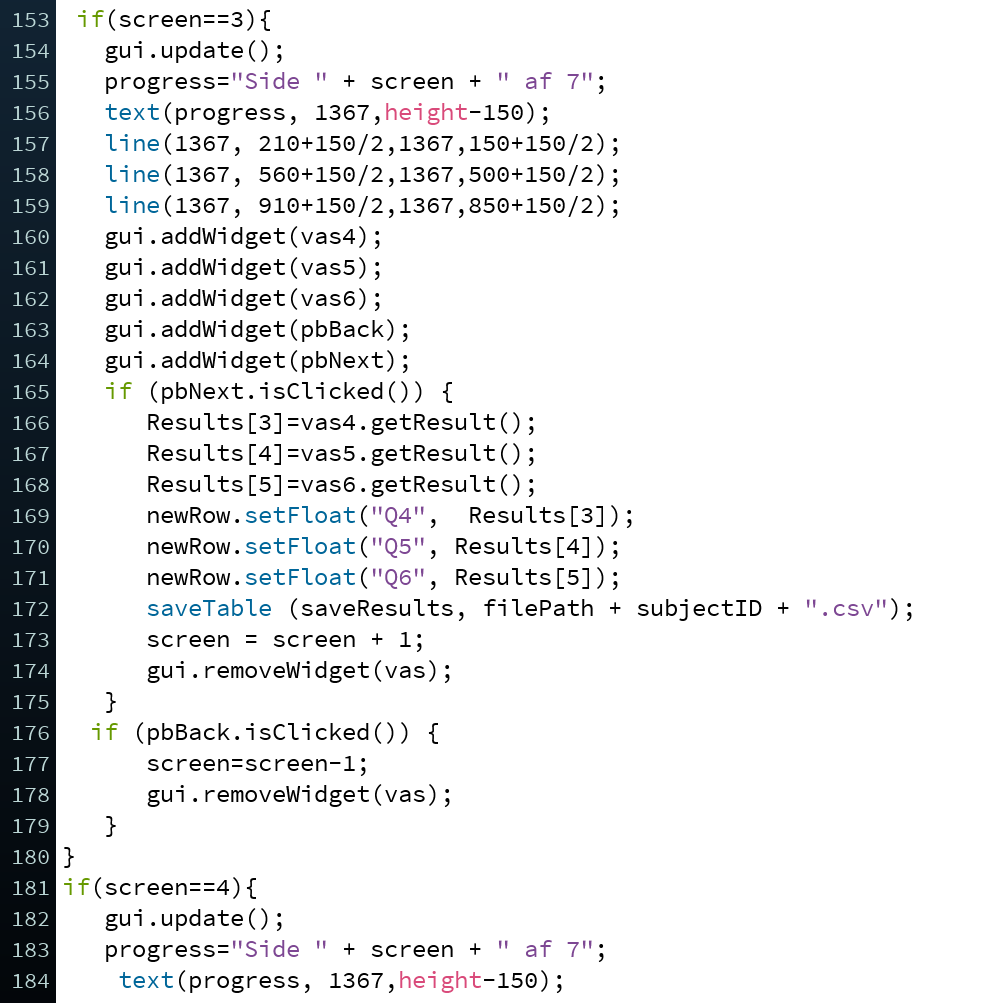
\includegraphics[width =\textwidth]{Figure/VASProgram/Screen} 
\caption{Udpluk af koden, som viser hvordan et skærmbillede sættes op og hvordan der navigeres mellem forskellige skærmbilleder.}
\label{fig:Screen}
\end{figure}
\noindent
%
Samme fremgangsmåde er anvendt til alle skærmbilleder med skalaer. Når der trykkes \textit{Næste} på det sidste skærmbillede med skalaer, skiftes der til en side hvor der står: \textit{Tak for hjælpen}, jævnfør linje 304-308 på \autoref{fig:Tak}.
%
\begin{figure}[H]
\centering
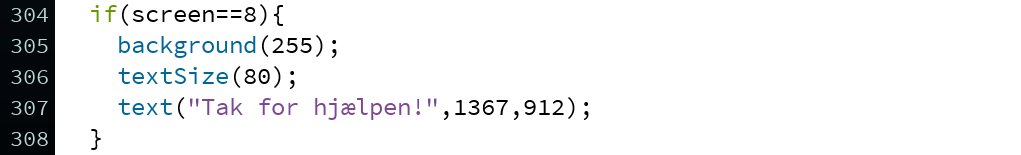
\includegraphics[width =\textwidth]{Figure/VASProgram/Tak} 
\caption{Udpluk af koden, som viser hvordan det sidste skærmbillede sættes op.}
\label{fig:Tak}
\end{figure}
\noindent
%
På \autoref{fig:VASEksempel} forefindes et eksempel på én af de syv sider med skalaer testpersonerne præsenteres for, hvor de forskellige GUI elementer fremgår. 
%
\begin{figure}[H]
\centering
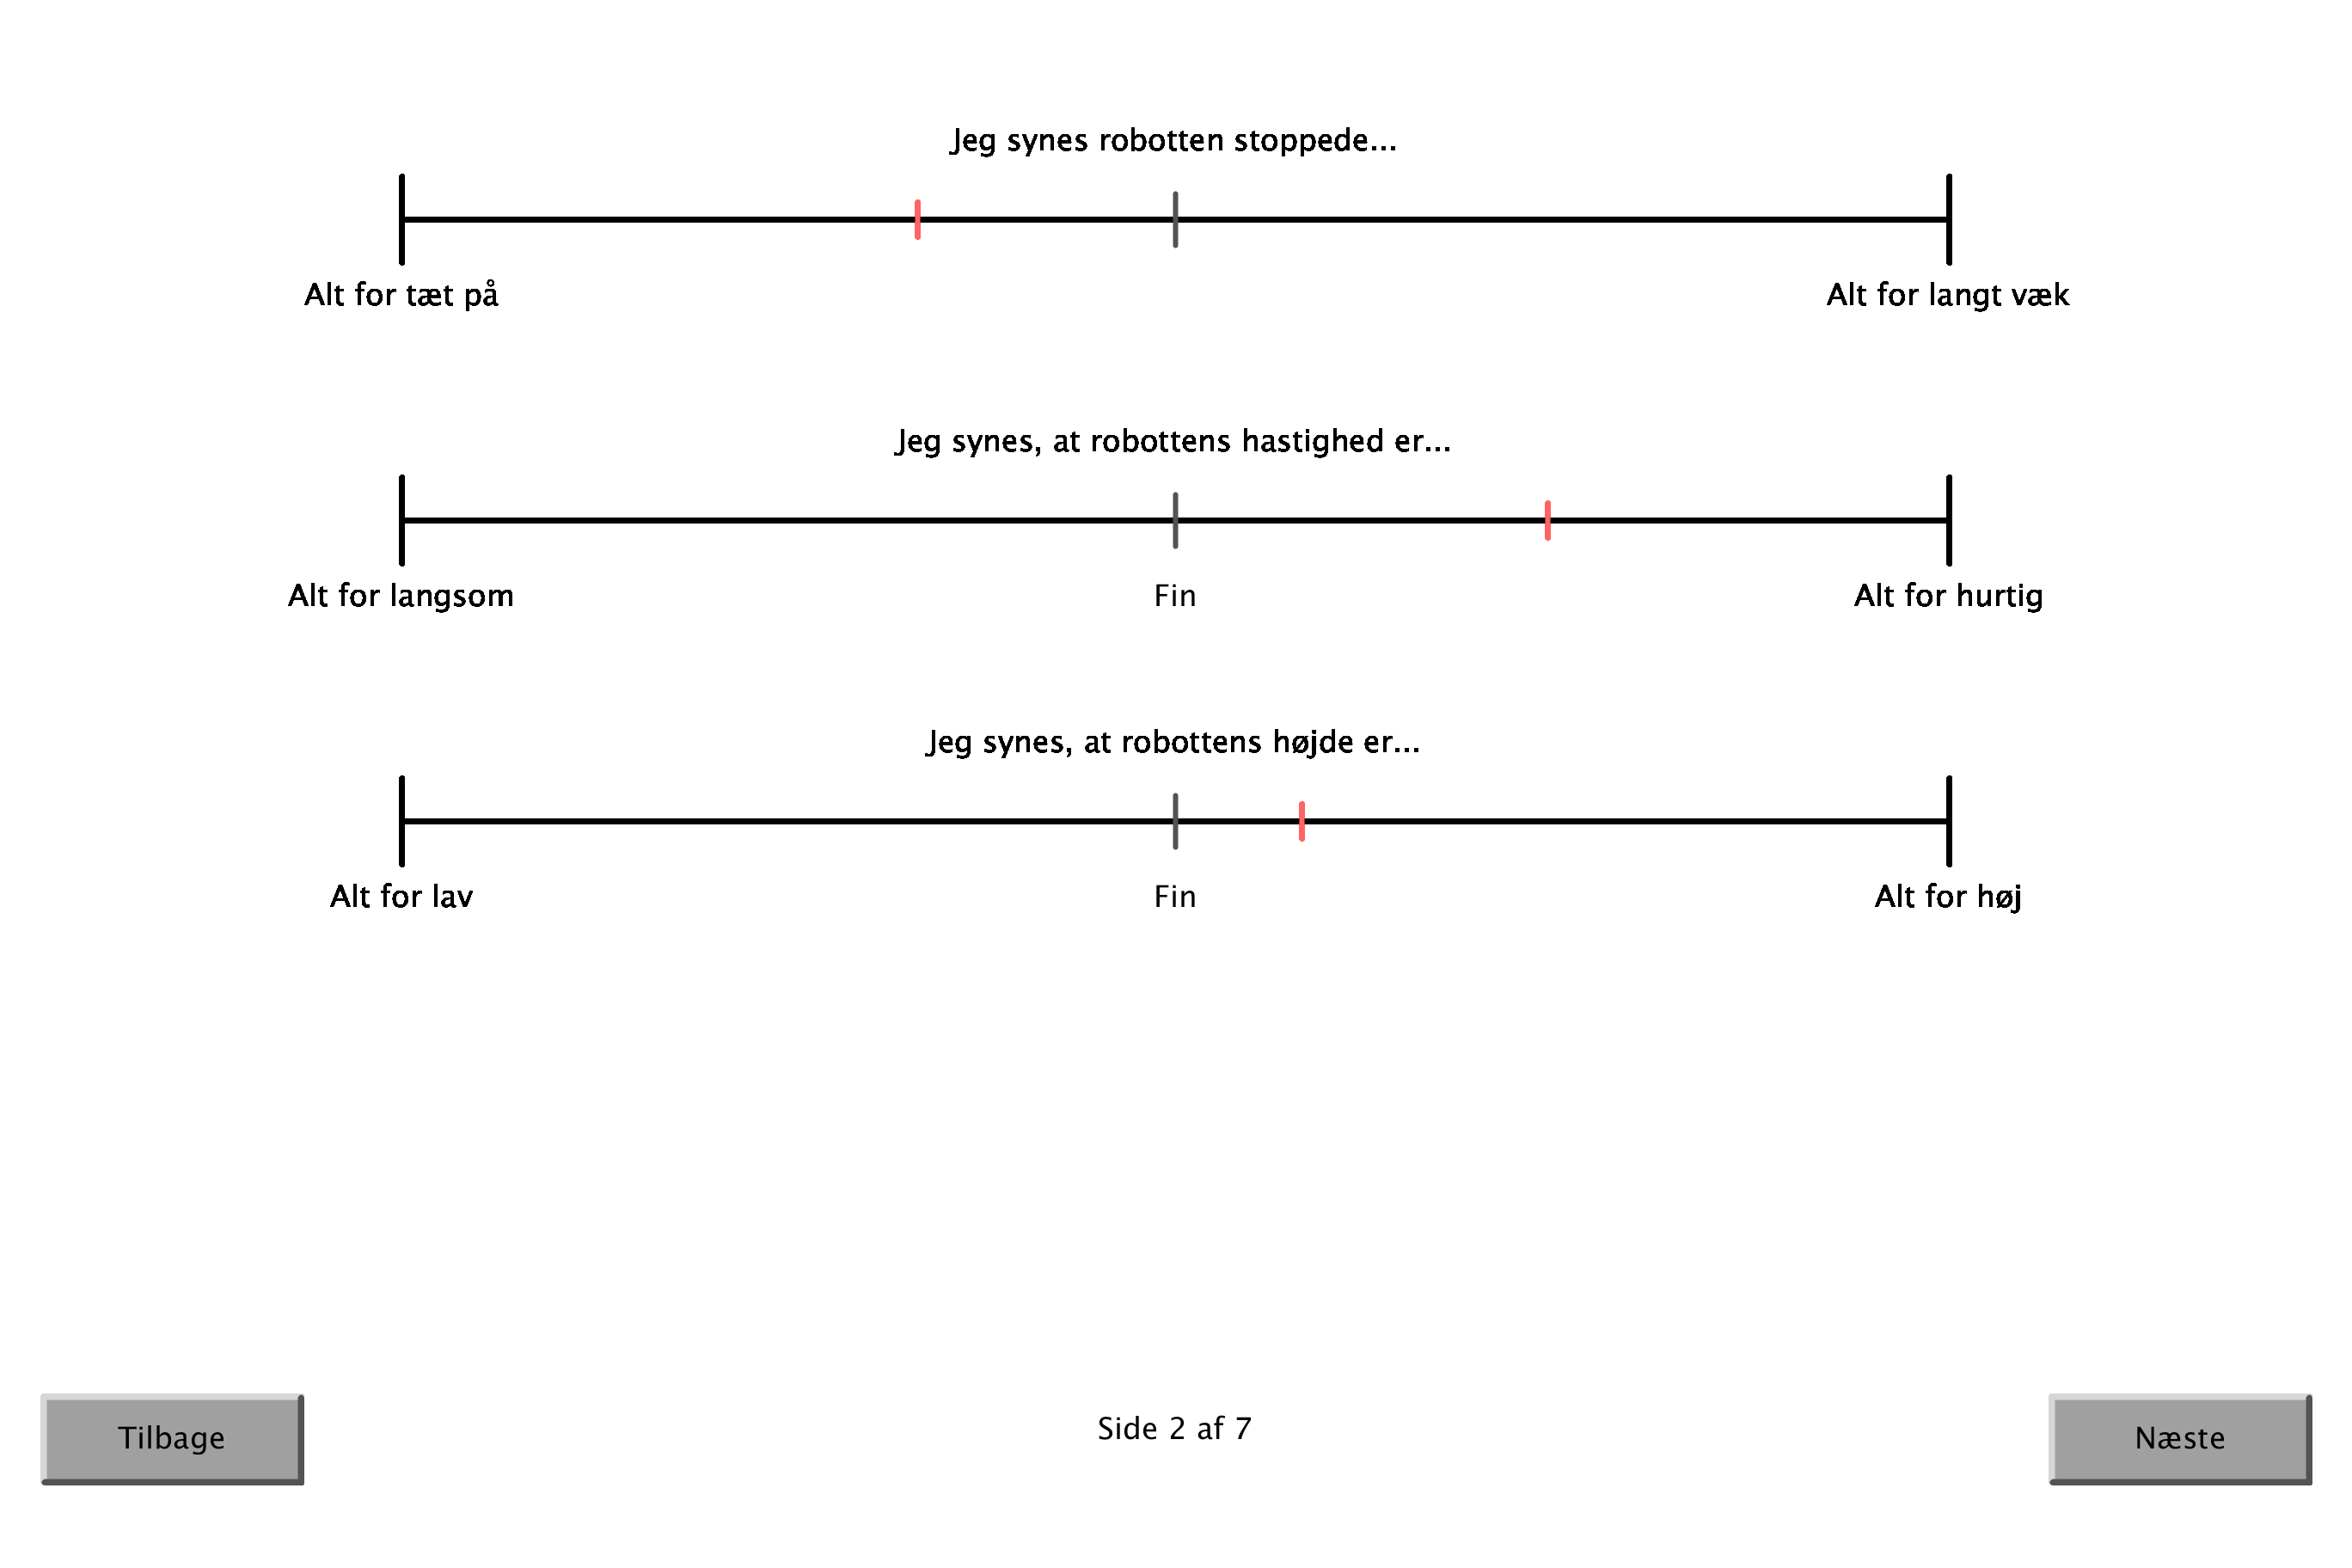
\includegraphics[width =\textwidth]{Figure/VASProgram/VASEksempel} 
\caption{Eksempel på et skærmbillede testpersonerne præsenteres for når de evaluere interaktionen med robotten. De røde markeringer afspejler testpersonen respons.}
\label{fig:VASEksempel}
\end{figure}
\noindent
%
Programmet bærer kraftigt præg af, at det blev udviklet i sidste øjeblik, grundet tidspres. Det havde derfor nogle fejl og mangler, som med fordel kan udbedres til en anden gang. Herunder opsummeres de problemer som blev opdaget og eventuelle løsningsforslag til, hvordan det kan optimeres. 

Det er muligt for testpersonerne at gå videre uden at angive en respons på de præsenterede skalaer. Det kan løses ved at tjekke om data er gemt for skalaerne på det nuværende skærmbillede og bruge det som en betingelse for at \textit{screen} kan øges med 1.

Programmet skriver 0 når der ikke bliver angivet en respons. Ved at løse problemet med at testpersonerne gik videre uden at svare, forsvinder dette problem også, da der aldrig vil være ubesvarede skalaer. Alternativt kan det vælges at skrive \textit{NaN}, hvis ikke testpersonen har angivet sin respons.

Programmet reagerer dårligt på tryk. Problemet skyldes sandsynligvis at programmet er en smule ineffektivt og bruger meget processorkraft på at læse kode, som ikke bruges på det pågældende skærmbillede. For at optimere det, kan der med fordel laves en PDPGUI for hvert skærmbillede, frem for at slette de gamle widgets og loade de nye hver gang. Endvidere burde \textit{while-loops} anvendes for hvert skærmbillede, frem for \textit{if-statements}, så computeren ikke skal gennem hele koden i hver iteration, men kun skal læse den kode, som bruges på det tilstedeværende skærmbillede.\blankline
%
Det samlede program fremgår af \fullref{ElektroniskBilagProgram}.
